\section{Experimenting with Reaching}

\subsection{Creating a Policy}
The next step was to create a policy network. As I am mainly working on imitation learning -and specifically behavioural cloning- from demonstrations provided by the system, my network needs to be able to ingest these demonstrations and generate actions in the action space of the robot. Following the earlier parameters of a demo, I created the following network, Figure \ref{fig:policy-arch}. This takes in the given wrist rgb image and extracts features, which are then interpreted into a $8$ dim vector of \textbf{float}s as an action. First $7$ corresponding to the $7$ joints of the \emph{Panda} robot, and holding a velocity value for them, while the final value is the gripper state, $0$ meaning closed and $1$ meaning open, which is clamped by the movement system under the hood.

\begin{figure}[h]
  \centering
  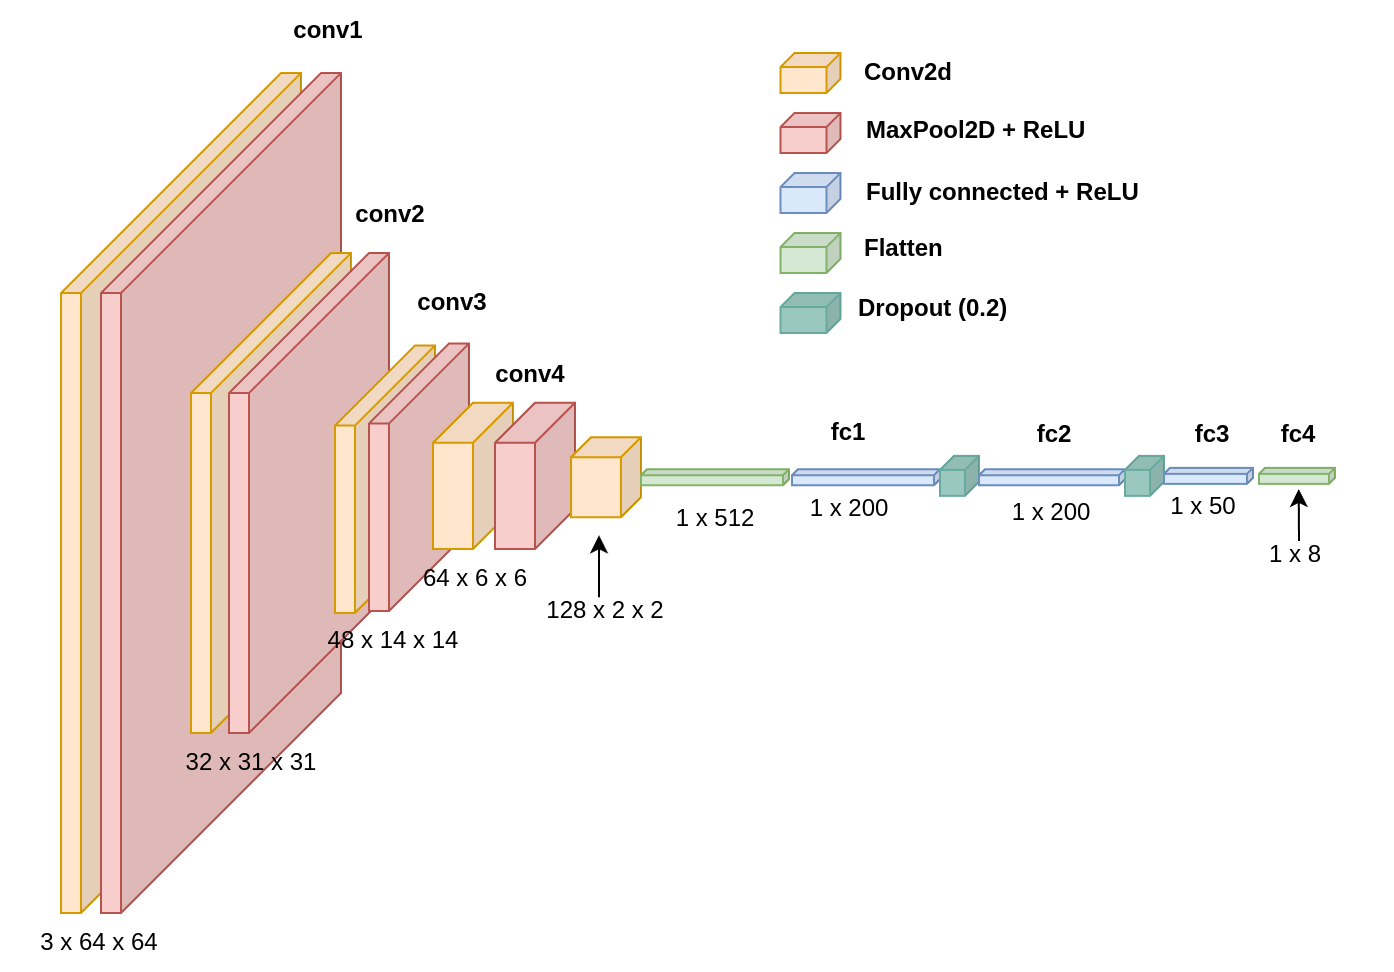
\includegraphics[width=0.6\textwidth]{assets/early-work/cnn-encoder-policy-head.png}
  \caption{Simple Policy Network Architecture}\label{fig:policy-arch}
\end{figure}\todo[color=blue]{ius the quality bad? reuload or reexport the xmml is in assets}

Along with the policy the second most important of any ML workload is the way the data us regularised, processed, and loaded into the system for training or testing.

\subsubsection{Data Processing}\todo{talk about rgb transforms? uniforming etc, or remove not sure}

\subsubsection{Data Loading}
I followed a simple flattening approach for loading the data into the system. Using PyTorch's \textbf{Dataset} and \textbf{DataLoader} classes I created a dataset that can take in a raw list of demonstration, then flattens its observations into a tensor of shape \(\langle 3,~64,~64 \rangle \) (permuted from the usual \(\langle 64,~64,~3 \rangle \) for images due to Torch conventions of convolutional networks and where they expect the channel  dimension). Then the dataset makes individual observation indexable along with their corresponding action labels. Types given as:\mintinline{python}|DemoObsDataset: tensor[tensor[3,  64, 64], tensor[8]]|. Then the loader can manage the shuffling and batching as usual. Initially I kept the data unshuffled, to keep the data in its sequential form. While keeping the batch size as the demo length. This is because currently I am trying to overfit the network to the single demonstration given to it to gauge how long to train my networks for

\subsection{Initial Observations}
Starting with the 3 static versions of the task, where the target is placed as shown in \ref{fig:no-obs-3-views} seen from the wrist cameras. I wanted to get an idea of how to tune the policy parameters. While understanding the relationship between training length and varying observability of the target.

\begin{figure}[htbp]
  \begin{subfigure}{0.3\linewidth}
    \centering
    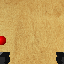
\includegraphics[scale=0.4]{../fyp/assets/demo-trials-no_obs/tasks/static-tasks-camera/initial-obs-side_l.png}      
    \caption{Left Side}
  \end{subfigure}
  \hfill
  \begin{subfigure}{0.3\textwidth}
    \centering
    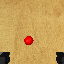
\includegraphics[scale=0.4]{../fyp/assets/demo-trials-no_obs/tasks/static-tasks-camera/initial-obs-central.png}
    \caption{Central}
  \end{subfigure}
  \hfill
  \begin{subfigure}{0.3\linewidth}
    \centering
    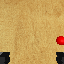
\includegraphics[scale=0.4]{../fyp/assets/demo-trials-no_obs/tasks/static-tasks-camera/initial-obs-side_r.png}
    \caption{Right Side}
  \end{subfigure}%
  \caption{Three variations of the reach task with the obstacles sometimes out of view}\label{fig:no-obs-3-views}
\end{figure}

I tested multiple epochs of training with the simple policy and recorded the final distance to the target at the end of their episode. The episode length is determined by the demo lengths, which I defaulted to the maximum, will also try mean, as keeping a static episode length doesn't make sense (especially on later tasks where the demonstration episodes can drastically vary in length)

The success of the tasks are wired to reaching the target in the simulator and will send a \emph{DONE} signal if it is reached. This happens around $0.12$ metres to the target. I have also observed the target will reach a very close distance but it won't trigger the detection in Coppelia, I think this must be a bounding box issue, wither the dummy objects that are doing the collision detection are missing each other, or the polling rate in the simulator is not frequent enough to detect this change. Either way, I added a way to count closeness into success if it were close enough.

\subsubsection{Static Tasks}
Testing on the static versions of the task, a simple policy with training around $20$ to $100$ epochs seems to do the job well, see Figure \ref{fig:rno-static}. And this is mostly because without variation in position simple Behavioural Cloning can be employed by overfitting to the data given. 

As I trained for longer it seemed to overfit early move really slowly at the start of the episode, wasting steps and ending up far from the target. Curious observation is \todo[color=purple]{} the central tasks behaves better at higher epochs which I believe is not necessarily because of visibility (the \emph{conv} features are not necessarily guiding anything with $1$ demo) but rather the centrality, as it is right above the gripper a simple downward bias allows the arm to easily get close to the target.

\begin{figure}[htpb] % htpb allows all placement
  \centering
  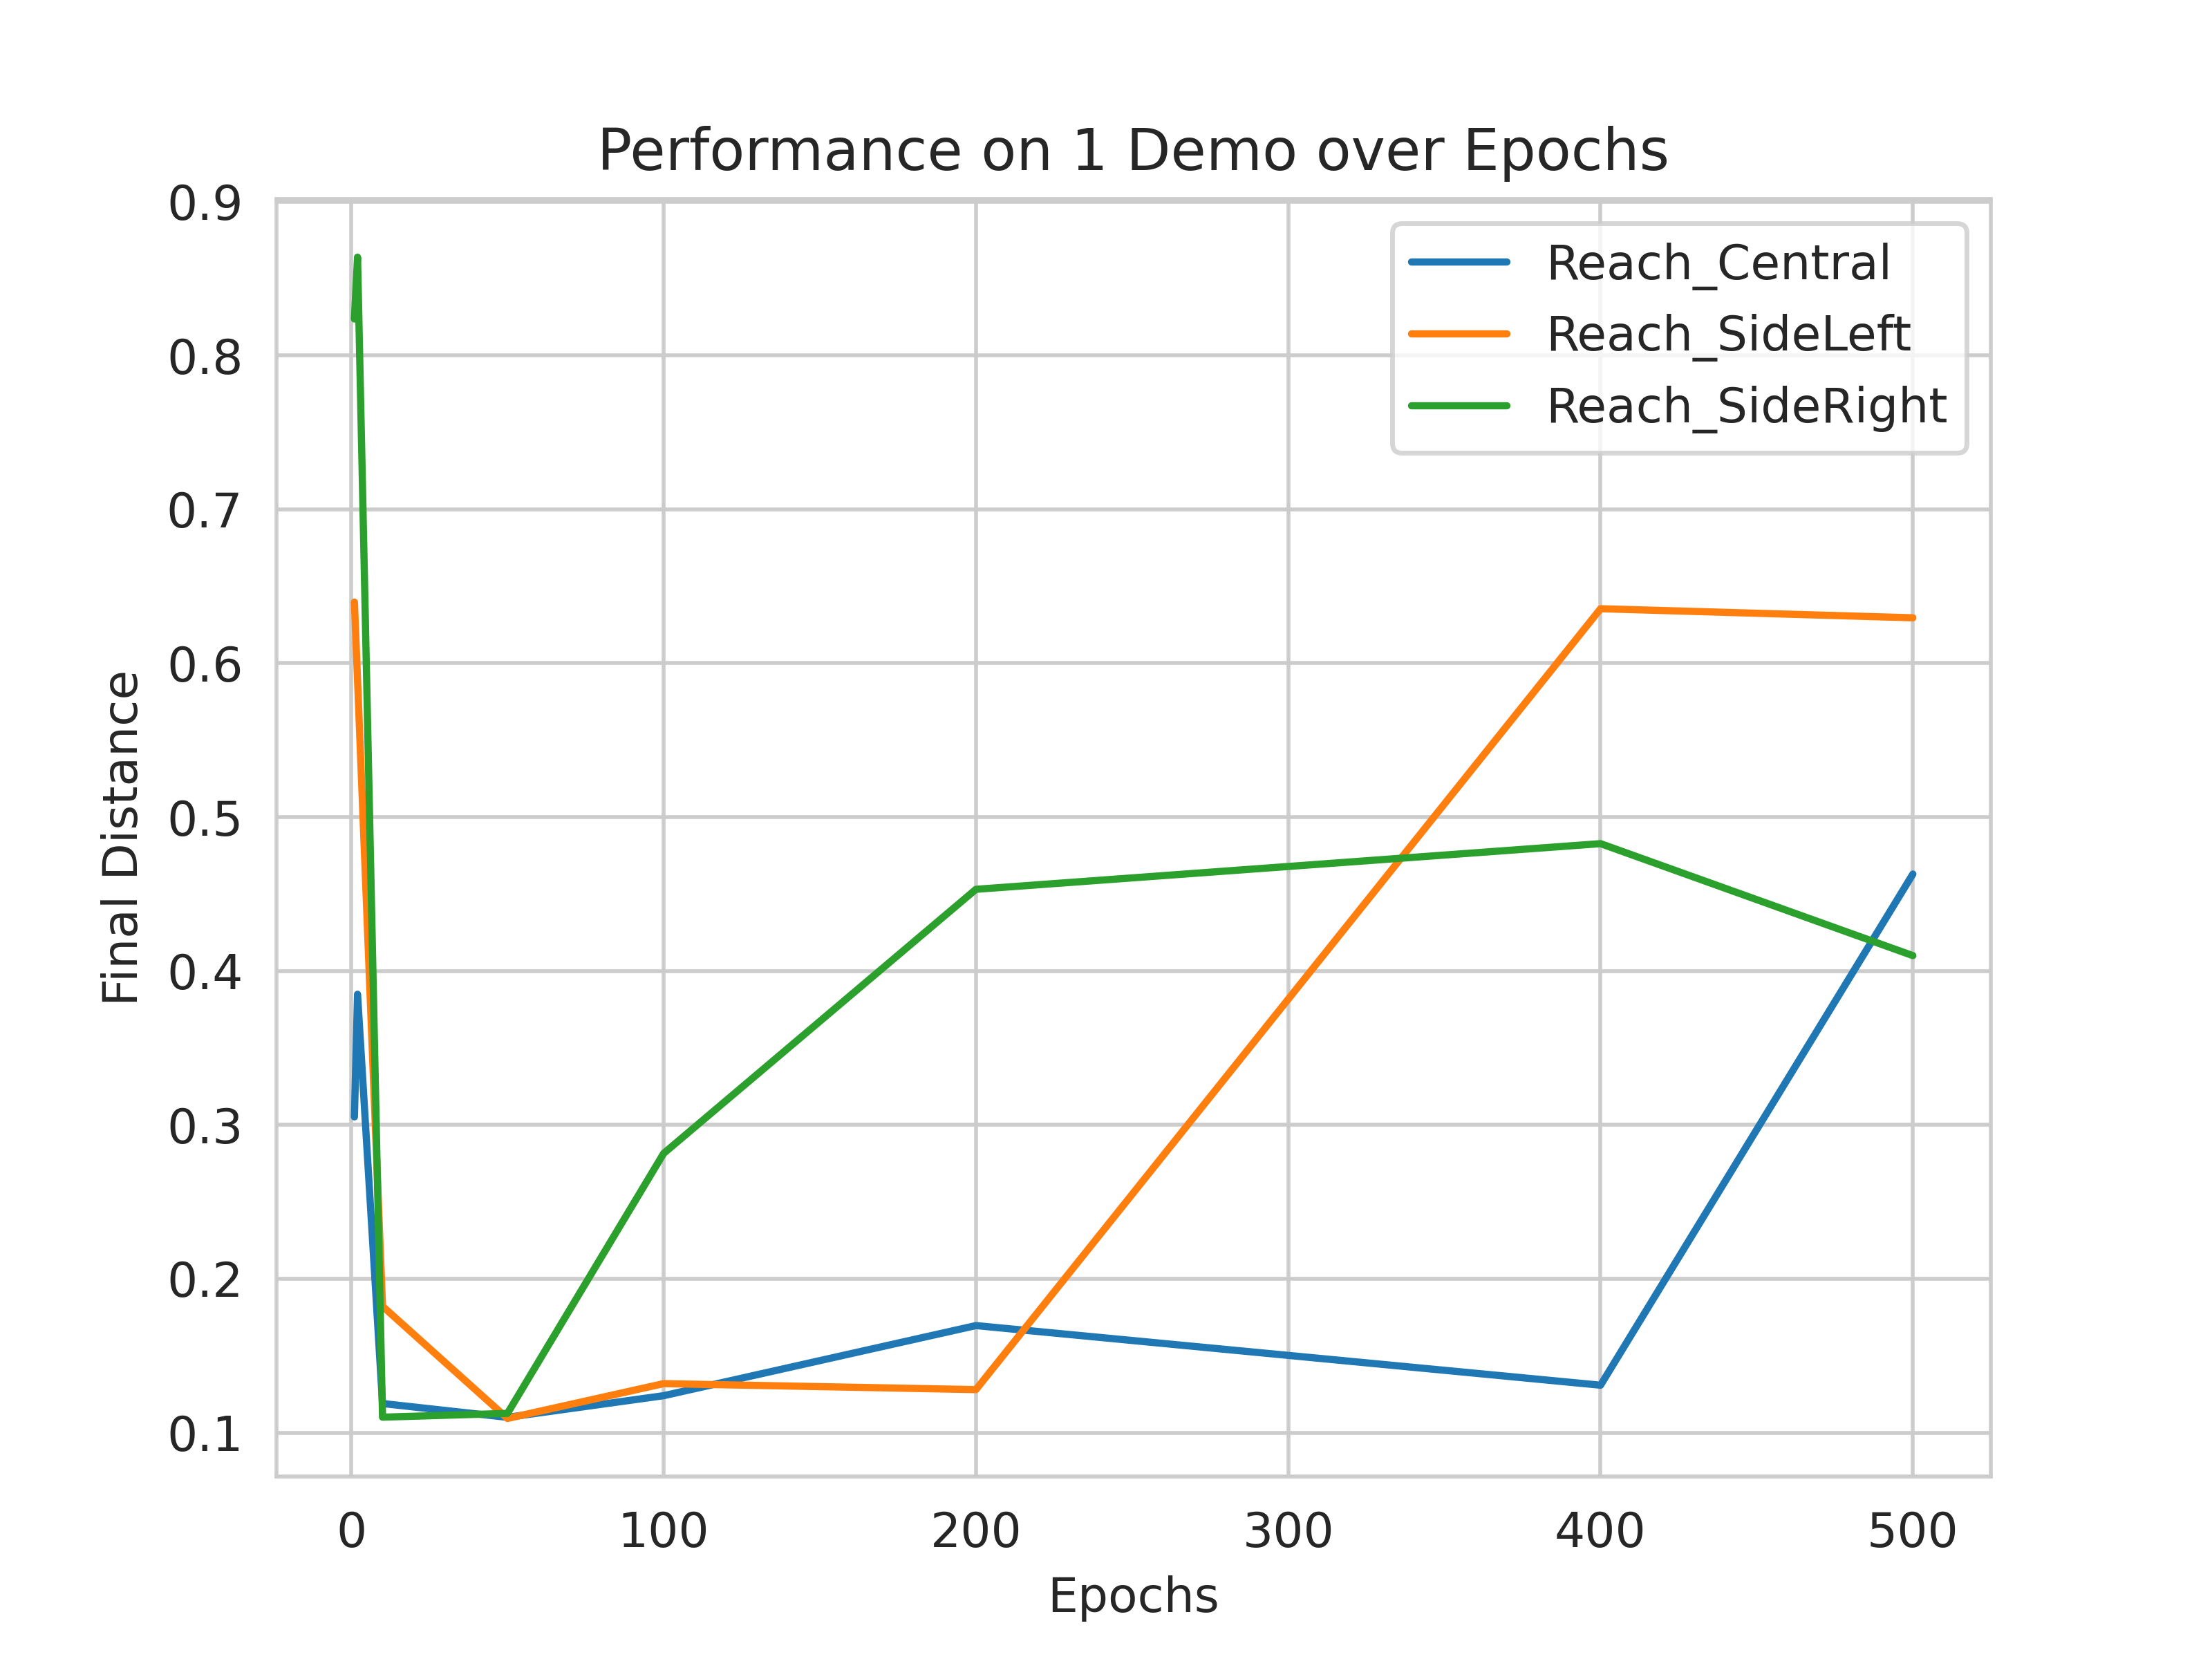
\includegraphics[scale=0.5]{assets/cam-comb/reach-no-obs/rno_static.png}
  \caption{Epoch experiments with the static tasks using a single demonstration}\label{fig:rno-static}
\end{figure}

\subsubsection{Placing Randomly}
To test generalisability, I created a dynamic version of the task, where the target is now randomly placed within view (not necessarily always fully within view, but at least some parts are visible). This is achieved by using a \verb|SpawnBoundary| and randomly sampling the location of the target withing this for every new variation of the task, or for every new episode. Which can be seen in Figure \ref{fig:reach-no-obs}, the white dotted box being the boundary. This boundary is not rendered in the simulation visually. This guarantees variety in demonstrations as well as helps us create a generalisable policy.

\begin{figure}[htpb] % htpb allows all placement
  \begin{subfigure}{0.50\linewidth}
    \centering
    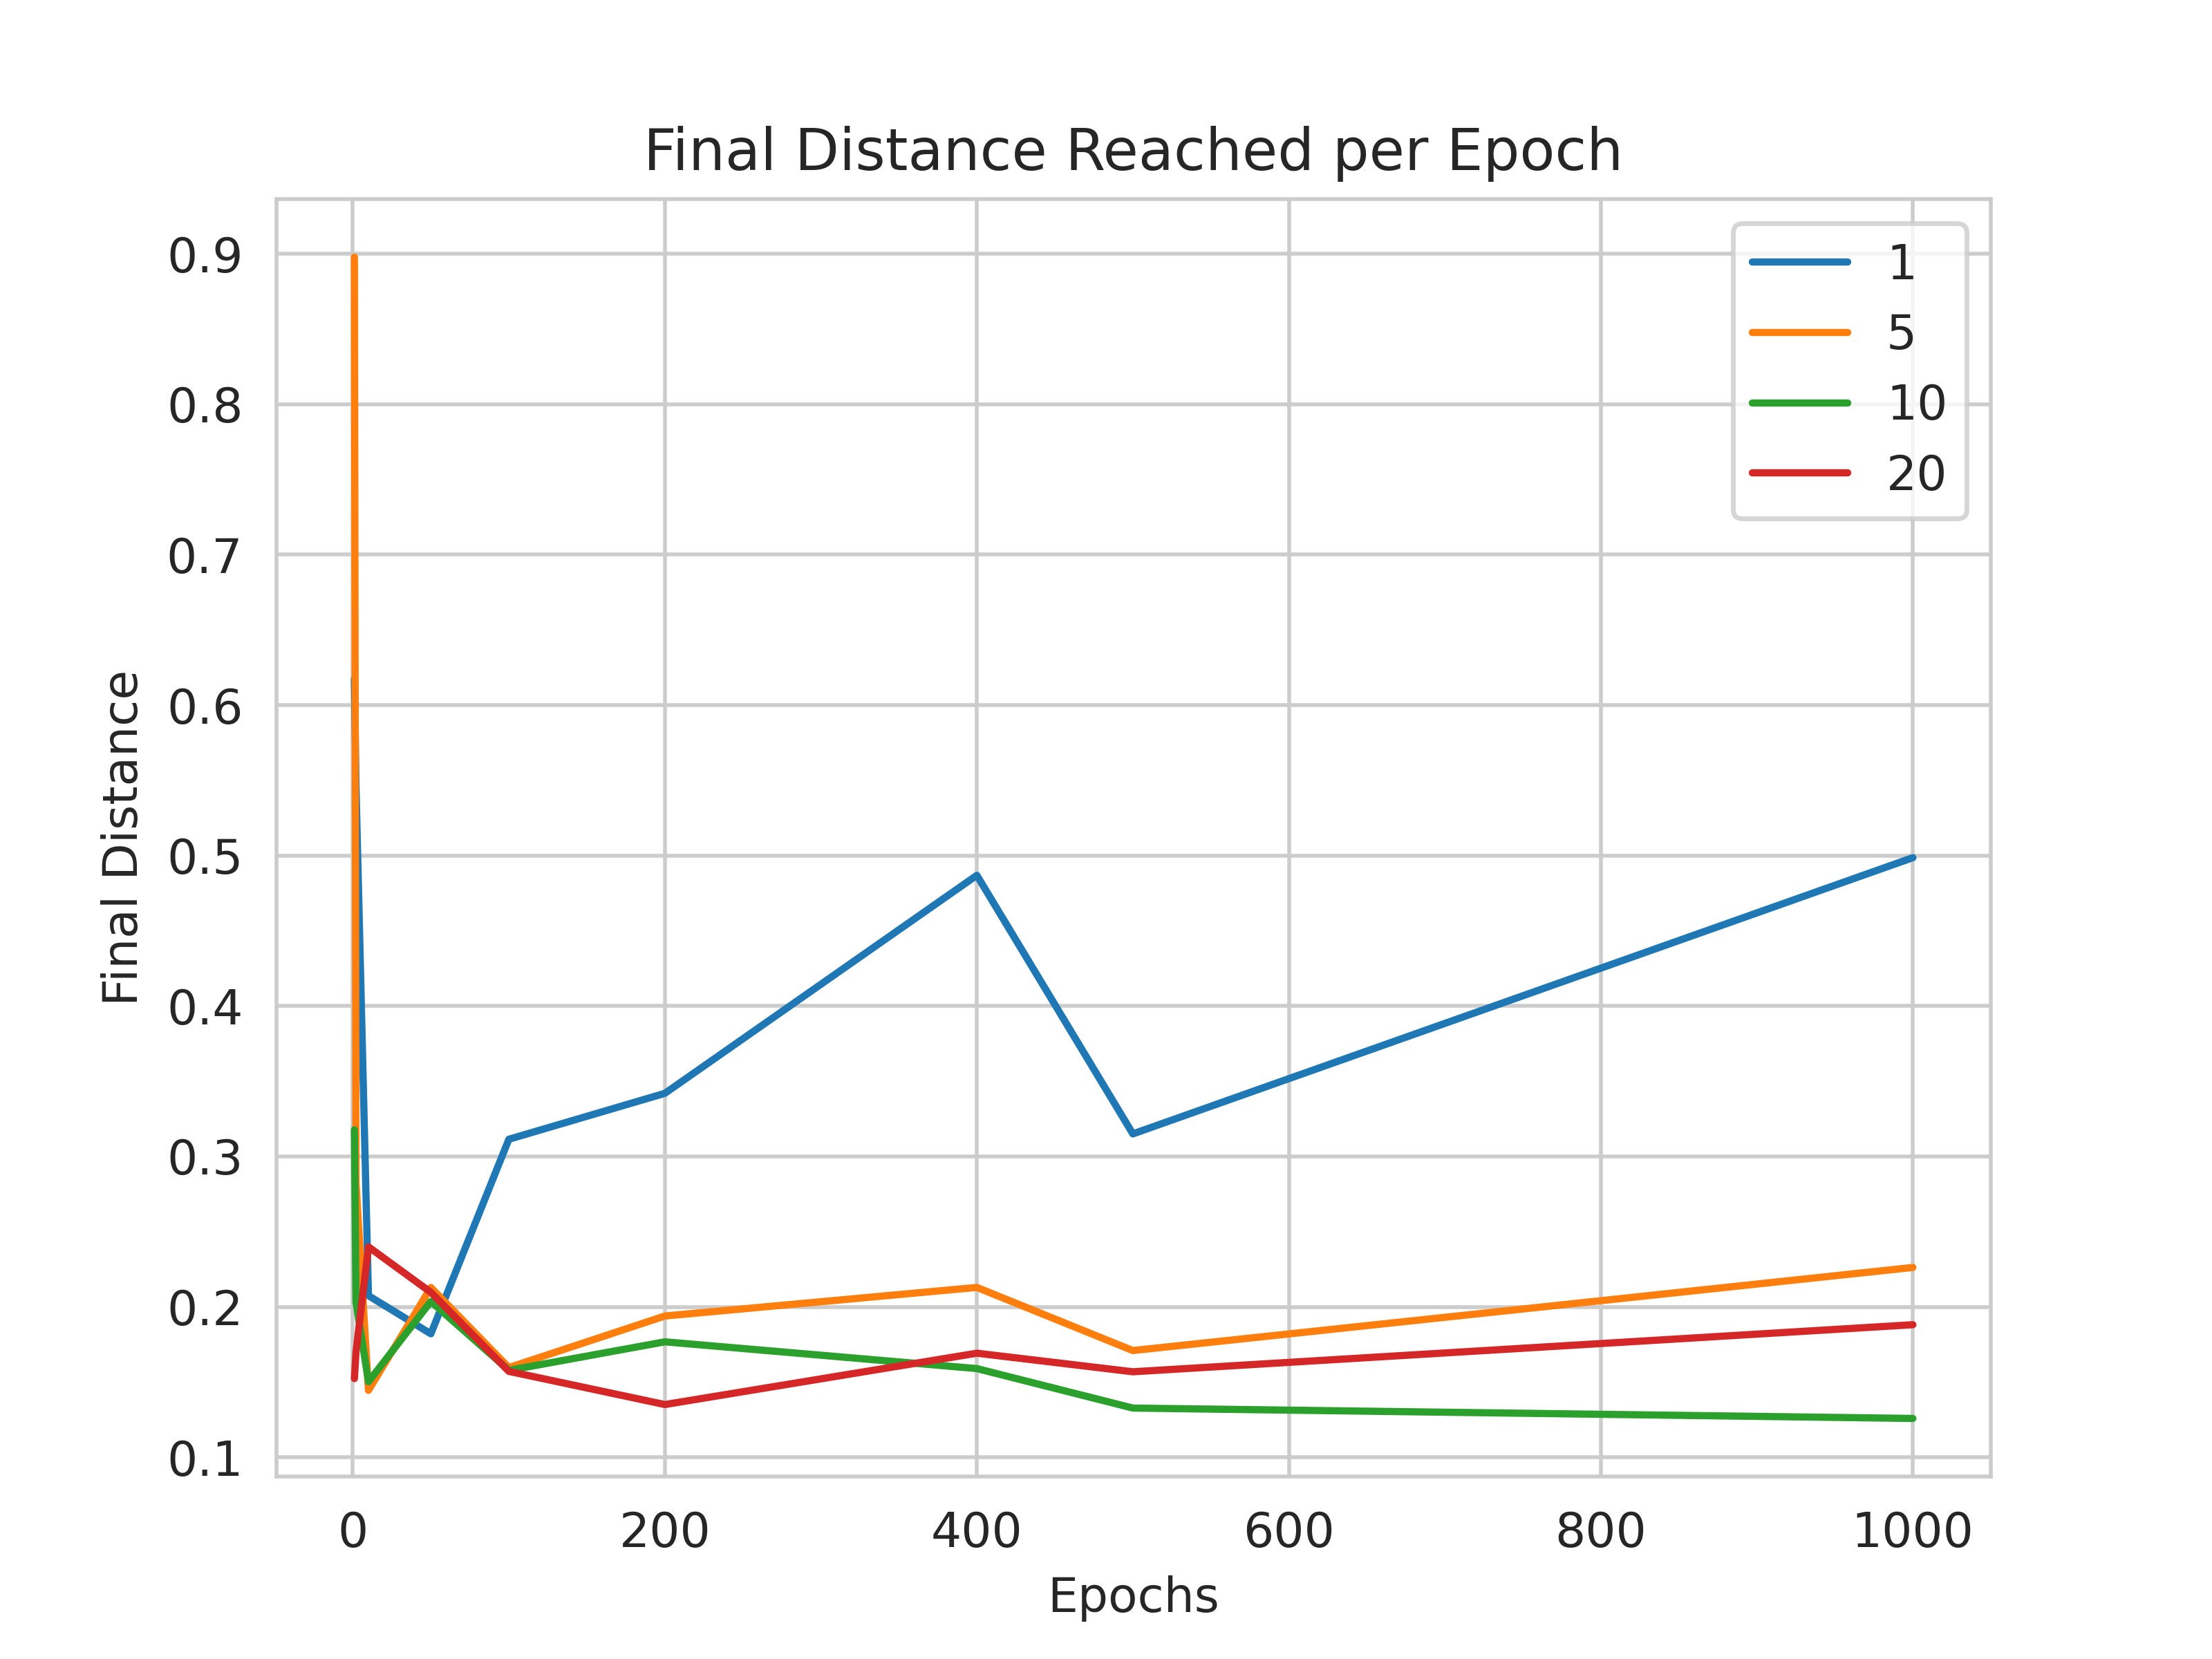
\includegraphics[width=\linewidth]{assets/cam-comb/reach-no-obs/rno_random-dist.png}
    \caption{Average Final Distance to Target}\label{subfig:rno-random-dist}
  \end{subfigure}
  \hfill
  \begin{subfigure}{0.50\linewidth}
    \centering
    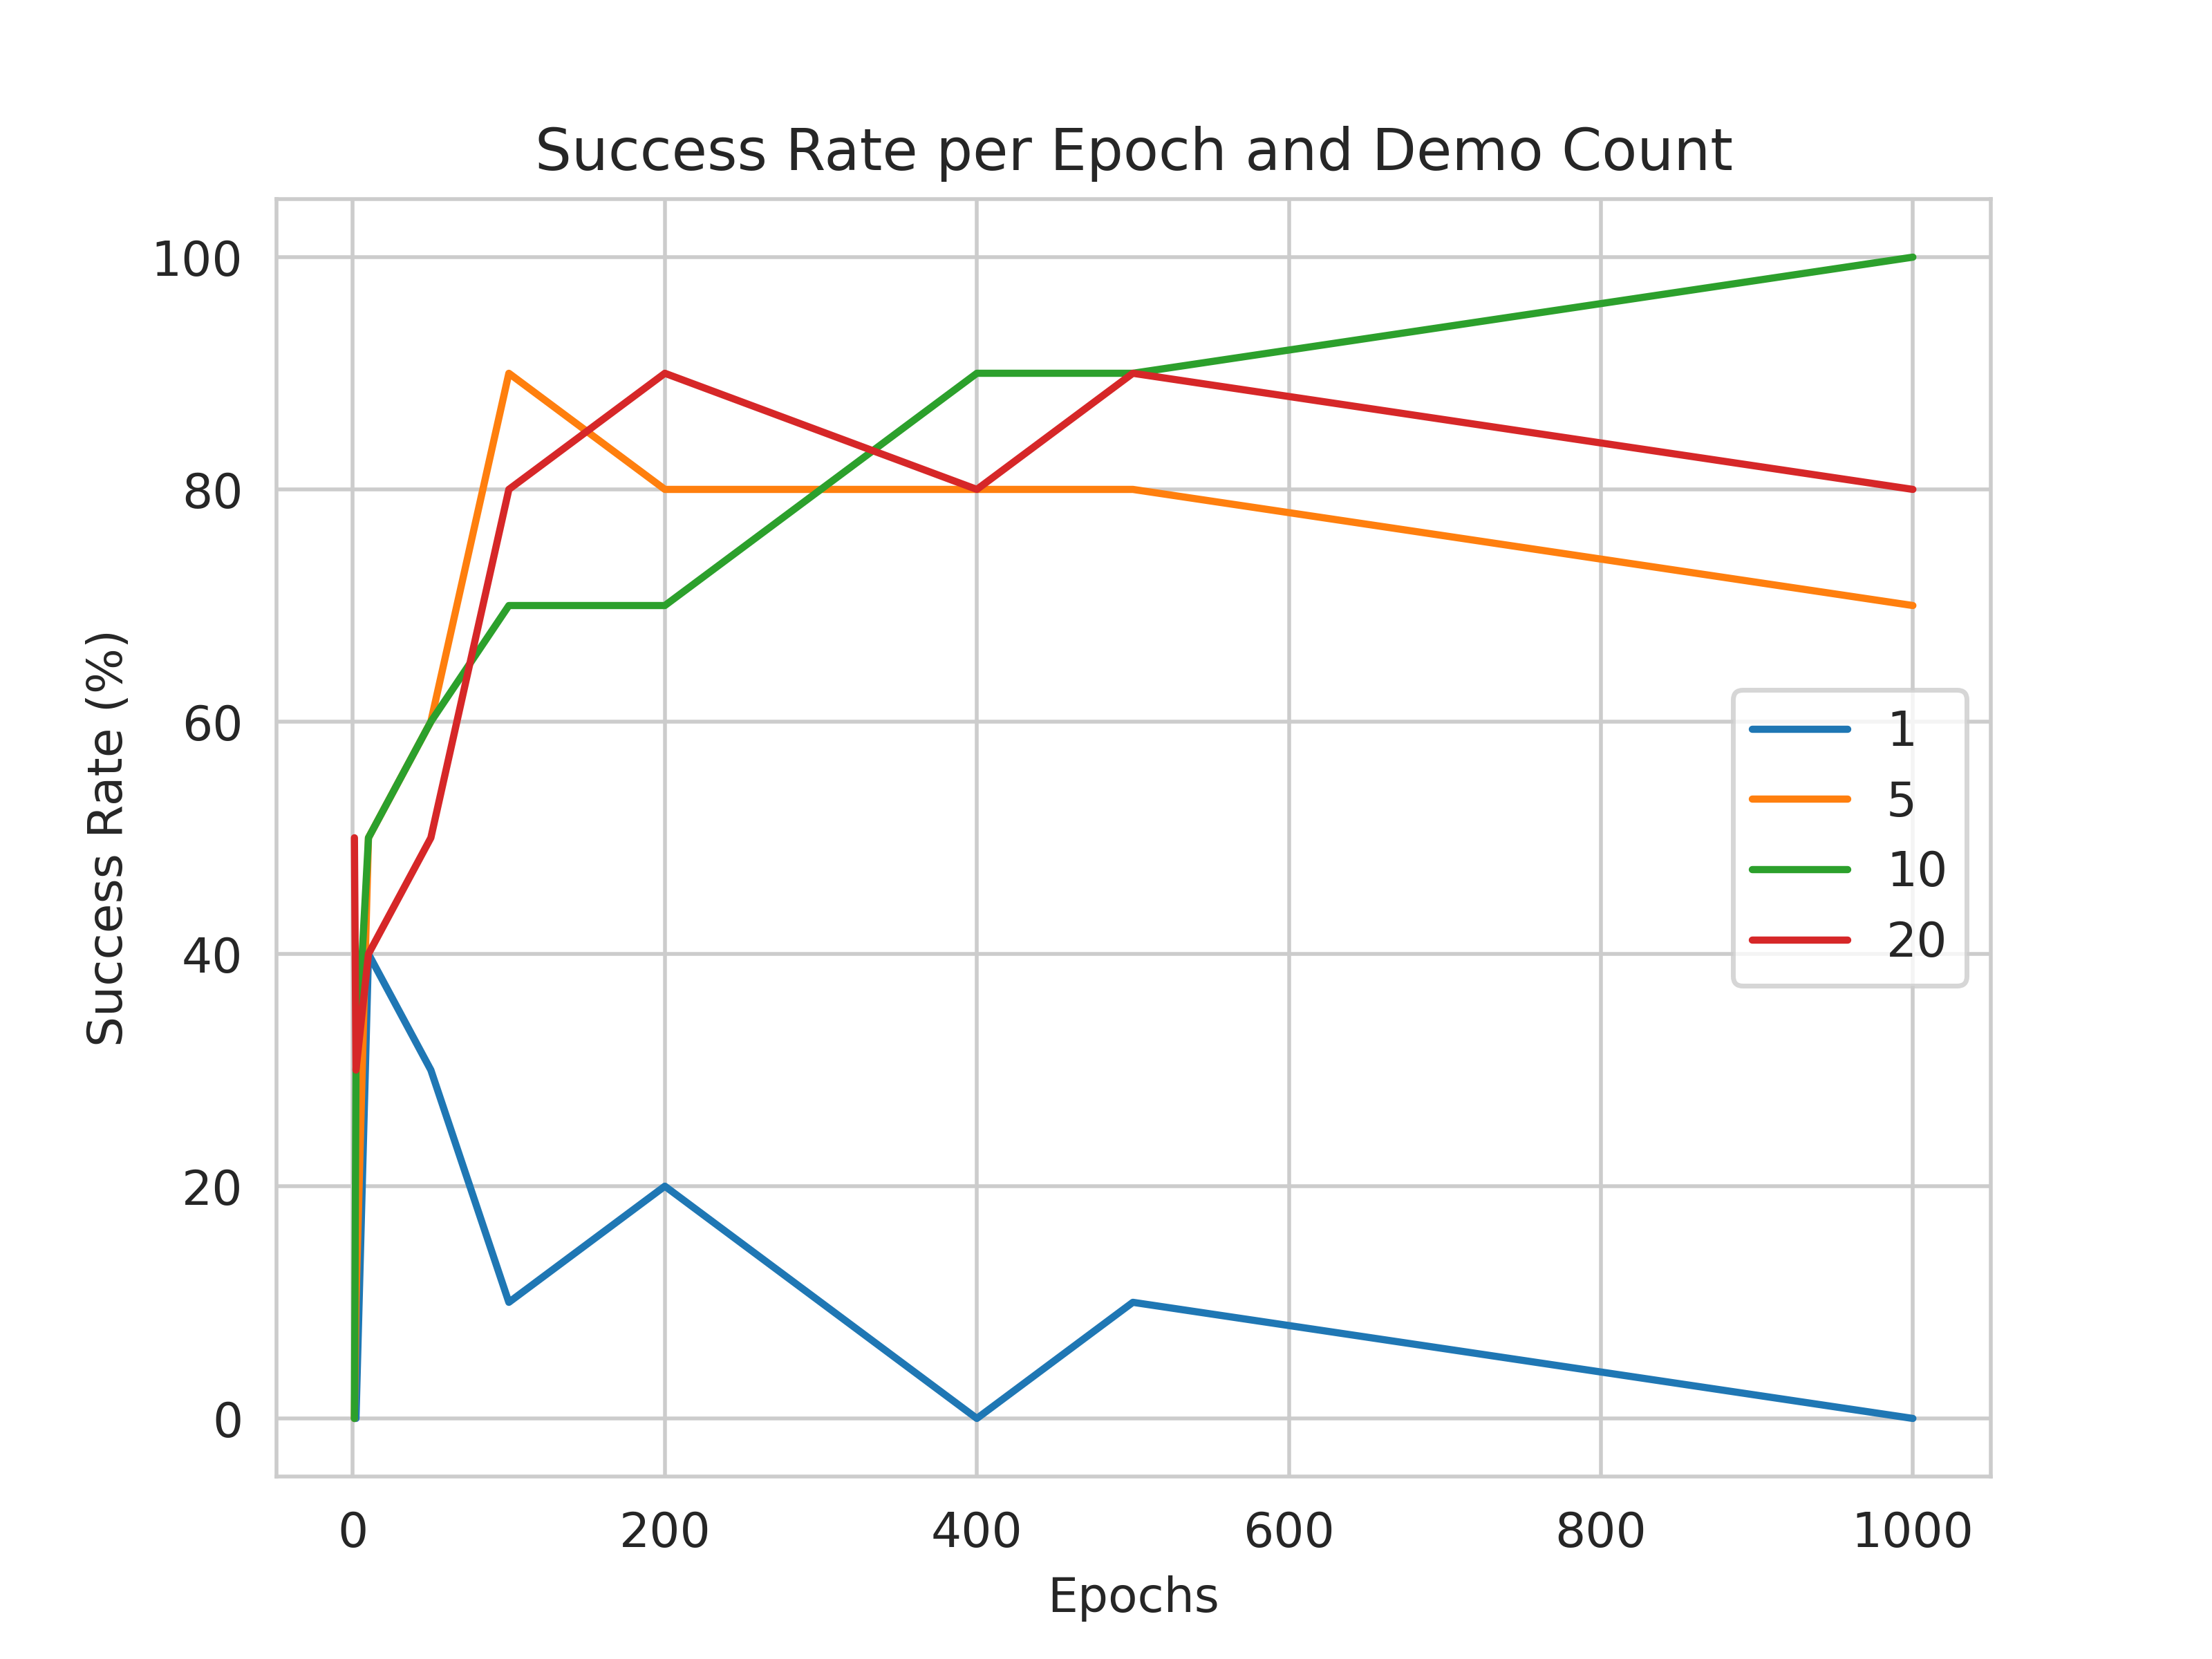
\includegraphics[width=\linewidth]{assets/cam-comb/reach-no-obs/rno_random-success.png}
    \caption{Success Rate (\%) for the $10$ Test Demos}\label{subfig:rno-random-success}
  \end{subfigure}
  \caption{Experiments with randomly placed target}\label{fig:rno-random}
\end{figure}

To run the random tests, shown in Figure \ref{fig:rno-random}, in a comparable manner I reused my set of demos that were created and saved earlier for this task for training. Then a set of 10 demos were randomly generated at the start and after the agent with the specific parameters were trained, I evaluated these policies against the test counterparts.

Looking at graph \ref{subfig:rno-random-dist}, we can see that providing more demonstrations helps the policy generalise better to random locations, where the sweet spots seems to be around 10 demos and around $500$ where the success rate (\ref{subfig:rno-random-success}) is quite high

\subsection{Camera Limitations}\todo[color=red]{reread and make sure it is a good starter segue to obs (maybe move these to after obs?), mention this under reachObs! MOVE}
I started this section by limiting the learning to only the wrist mounted camera, which works well for this specific unobscured task. Introducing some of the other RGB cameras, specifically the \verb|left shoulder| or the \verb|right shoulder| views, does not necessarily benefit the performance, see \ref{fig:rno-random-cams}. Conversely, we are increasing the training time by adding more channels to the convolutional layers, which can be considered a drawback.

\begin{figure}[htpb] % htpb allows all placement
  \begin{subfigure}{0.50\linewidth}
    \centering
    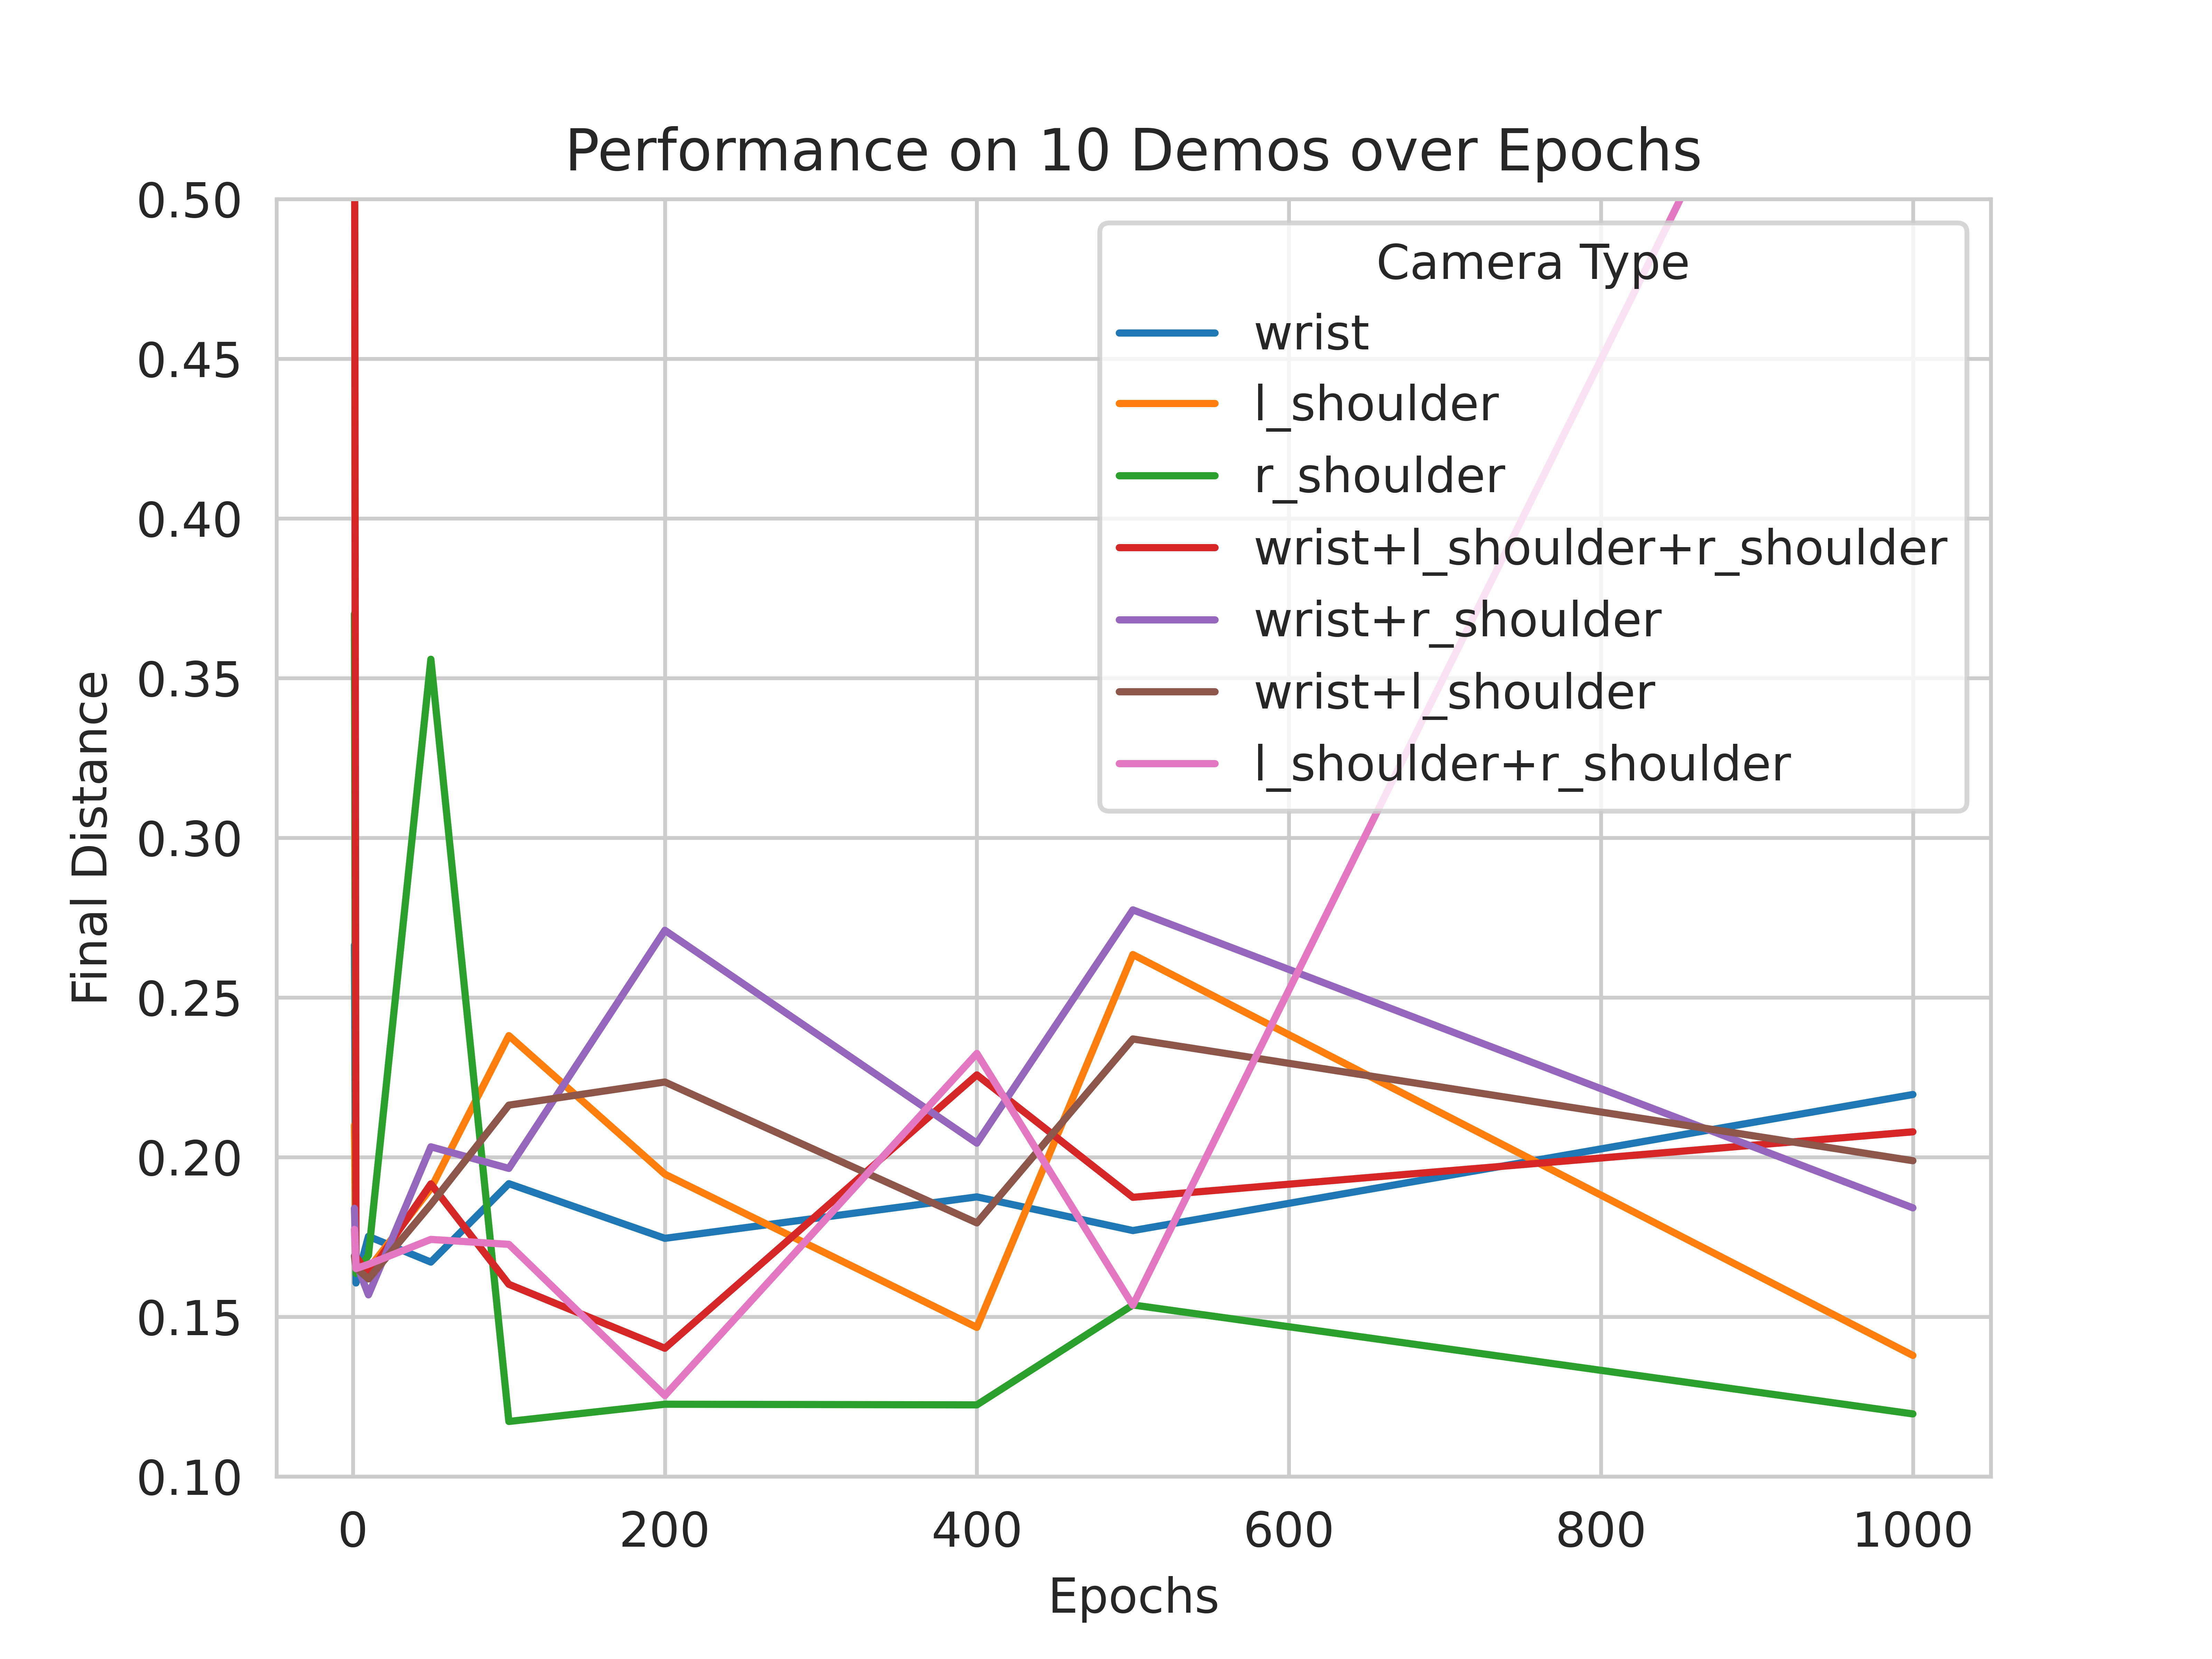
\includegraphics[width=\linewidth]{assets/cam-comb/reach-no-obs/rno_random-cams.png}
    \caption{Average Final Distance to Target}\label{subfig:rno-random-cams-dist}
  \end{subfigure}
  \hfill
  \begin{subfigure}{0.50\linewidth}
    \centering
    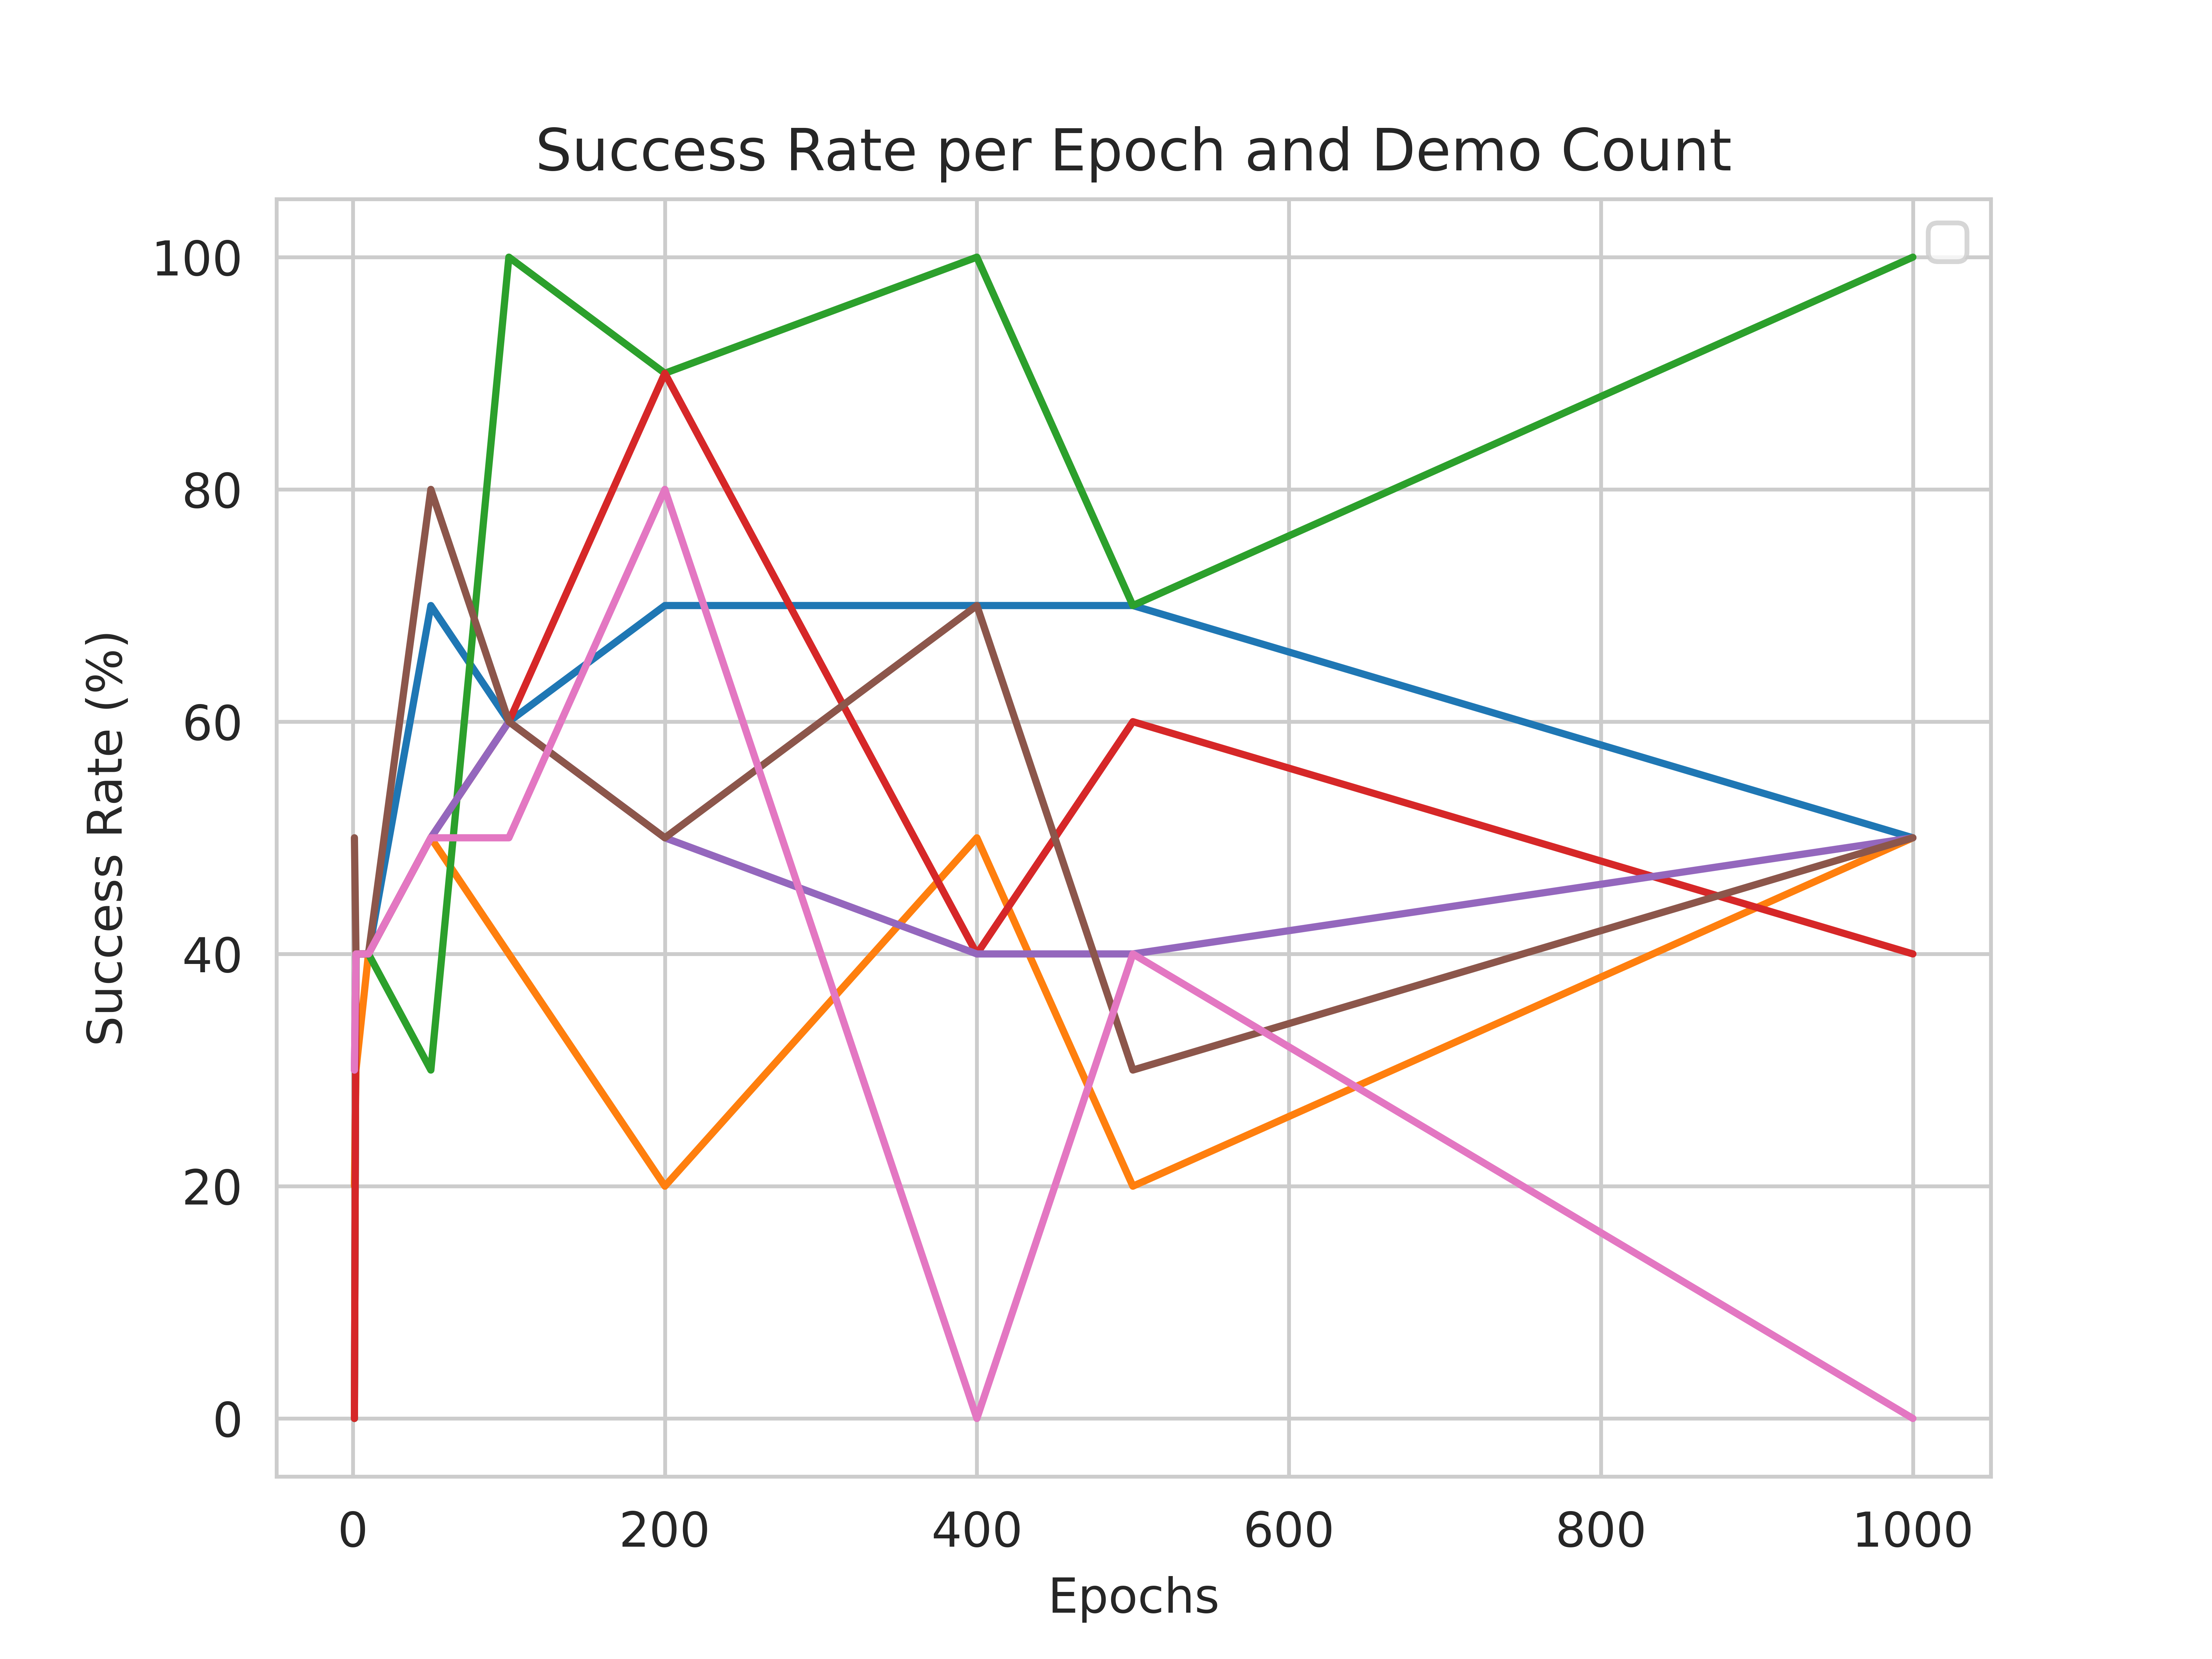
\includegraphics[width=\linewidth]{assets/cam-comb/reach-no-obs/rno_random-cam_success.png}
    \caption{Success Rate (\%) of the $10$ Demos}\label{subfig:rno-random-cams-success}
  \end{subfigure}
  \caption{Experimenting with multiple RGB cameras}\label{fig:rno-random-cams}
\end{figure}

Although the performance does not outright increase, we can clearly see that having a different point of view can sometimes drastically affect the quality of the learnt network and hence the action produced. \todo[color=purple]{}  \todo{need to actually talk about the numbers here refer to graph}

However, this is not to say all tasks will be immune to benefits from extra views. An important part of this project is to understand what is most important for a robot to observe in its given environment and task and how can it optimally leverage this data to solve a task better. And increasingly more complex tasks should benefit from abundance of information.

\subsection{Increasing the Toy Task Complexity}\todo{subsection to above?}
Complexity of tasks can be increased in two main ways:
\begin{enumerate}
  \item Introducing non-linearities to the environment to make a scene more challenging to traverse for an agent
  \item Increase the movement or the level of interaction of the task at hand
\end{enumerate}
I plan to do these mainly by introducing obstacles; which will guide me to understand what an agent needs to understand navigation. Secondly, I want to branch out to a grasping task, to increase the number of items of execution, to evaluate the capability of an agent to use its understanding to complete increasingly more complicated tasks.

\section{Reaching with an Obstacle}
To add onto the reaching task, I introduced an obstacle placing mechanism as well as randomly placing the target behind this obstacle, ensuring the agent doesn't learn where exactly target is by looking at just the obstacle\todo[color=purple]. See Figure \ref{fig:reach-obs-random} for how this task looks and the check \todo[color=green]{add appendix link, and code} for the backend wiring of the task.

\subsection{Creating the Task}
There are two versions of this task, I thought it might be interesting to randomise the object firstly dependently then independently on the obstacle. The `dependent' randomisation called \verb|ReachObs_Random| samples the obstacle, which in turn controls the spawn boundary of where the target can spawn in, meaning the target will always appear behind the obstacle albeit, edges of it can sometimes stick out. Conversely, the `independently' random version, called \verb|ReachObs_IndRandom|\todo{also add to appendix and link here}, keeps the target spawn boundary fixed, meaning the target can be anywhere in the visible workspace, but it is not necessarily always covered by the obstacle. I can see that this potentially can be useful to keep the dataset a bit more diverse, and allow the wrist camera initially observe the target sometimes.\todo[color=red]{use this somewhere, or hint back to it, maybe even to say there was no difference}

\begin{figure}[htpb] % htpb allows all placement
  \centering
  \begin{subfigure}{0.3\linewidth}
    \centering
    \includegraphics[scale=0.3]{../fyp/assets/task-pics/reach-obs/random-front.png}
    \caption{Front}
  \end{subfigure}
  \hfill
  \begin{subfigure}{0.3\linewidth}
    \centering
    \includegraphics[scale=0.3]{../fyp/assets/task-pics/reach-obs/random-side.png}
    \caption{Side (Left)}
  \end{subfigure}
  \hfill
  \begin{subfigure}{0.3\linewidth}
    \centering
    \includegraphics[scale=0.3]{../fyp/assets/task-pics/reach-obs/random-top.png}
    \caption{Top}
  \end{subfigure}
  \vfill
  \begin{subfigure}{0.45\linewidth}
    \centering
    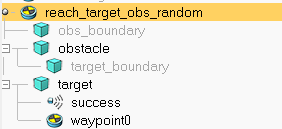
\includegraphics[scale=0.5]{assets/early-work/obs-random-scene-hierarchy.png}
    \caption{`ReachObs\_Random' Scene Hierarchy}
  \end{subfigure}
  \hfill
  \begin{subfigure}{0.45\linewidth}
    \centering
    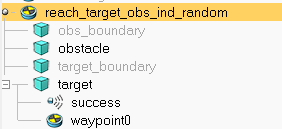
\includegraphics[scale=0.5]{assets/early-work/obs-ind-random-scene-hierarchy.png}
    \caption{`ReachObs\_IndRandom' Scene Hierarchy}
  \end{subfigure}
  \caption{Reaching Task with an Obstacle}\label{fig:reach-obs-random}
\end{figure}\todo[color=blue]{smaller?} 

\subsection{Experimenting with Views}\todo[color=red]{}

\subsubsection{Using same unchanged policy form ReachNoObs}
\todo{run the best params we have for the first one here with nothing changed}

\subsubsection{Understanding the Data Management}
\todo{mention switching to demo dataset}
\missingfigure{shuffling plots}
Talk about how the data is loaded and created and managed for the network, talk about shuffling mechanisms and what I've found etc. talk about \verb|shuffle_obs_in_demo| and the other one.

\subsection{Improvements}



\subsubsection{Wrist Camera Alone isn't Enough}
As expected this is where the single wrist camera started showing its shortcomings. The agent would easily move around the obstacle, however, would struggle to make the last steps in touching the target. This is mostly due to the fact that the demonstrations (which are provided by RLBench) are not necessarily pointing the wrist of the robot and hence the camera mounted there to look towards the target. This means that the behavioural cloning agent learns to to the swaying motion around a large grey body, however, is not aware of the obstacle, or even understand the task is related to reaching for the obstacle and depends on its visual cues. 

\todo{add graph of going around the obstacle but not quite reaching the target (wrist)}
\todo{show this with other combinations of cameras, comment on if the l/r without wrist can learn to go around the obstacle easily? maybe not, generalisation might be hard with no wrist}

From experiments I have realised that it learns to move around the obstacle easily, using simple behavioural cloning. However, getting the last nudge to actually reach the target is where it falls apart, especially in more realistic scenarios where the target is randomised behind the obstacle. For static placement behind the wall, the agent, expectedly is quite good. \todo{maybe explain or evidence this, plateaus aroudn the same distance value and watchig t heroot act comfirms this}

\subsubsection{Other Cameras}
So, we can confirm that the wrist camera alone is not sufficient \todo{ref}, and the combination of wrist and other cameras are almost always better as more coverage of the workspace guarantees less occlusions and more information the agent can work with to make decisions. It was clear that the wrist camera alone wasn't going to cut it unless it learnt to look towards the target.\todo[color=red]{looking at he target??}


\todo{talk about the policy using differnt camera inputs to blend and make informed choices? maybe some plots here showing if it is better or not?}
\todo{this is important for plan2 later, as that would depend on such a mechanism, hint and even link that from here}

\subsubsection{Implementing `Looking' into the Demonstrations}\todo{haven't done this yet}\label{ew-looking-at-target}
issues this is not easy might be working on this as a part of approach 2 later
Another solution might be to experiment with the demonstration system to make sure we are pointing the wrist camera (so, the hand of our robot) towards its target as a demonstration trajectory is calculated \todo{explain that this proved tricky and might not even be worth it}

If we can't implicitly encode the `looking' information through the demonstration that means we will have to inject this information into our agent some other way. Another way to make sure agent understands to look at the target is teaching it to actively seek out its target, either following previous works such as \todo{find some prior info tracking works add ref} where object priors are incorporated into the learning or with attention mechanisms that figure out what is important in a task without prior object information \todo{maybe reference this later}.  

\subsection{Attending on a Camera in Given Combination}
\todo{talk about the implementation of the }
\subsubsection{MultiCNN}
\todo{explaint the implementations, maybe connect to }
\subsubsection{SingleCNN}
I initially though to disconnect the convolutional network, thinking the information can be encoded per view and then fused together to assign better meaning to the given pose. However, with the same logic the scene is still the same scene and encoding features together means that the network will learn to \todo{find a nice way to say the network will learn its fusing in the conv layers. maybe make sure it can}